% Provenance (never printed): cycle 4 SVT/physique, "La planete Terre,
% l'environnement": uneven heating of the Earth, movements of the
% atmosphere, the global circulation and the climate zones; see
% sources/book1/PROVENANCE.md. Book 1, grade 8, chapter 2.
% Vocabulary guard: owns convection cell (atmospheric, descriptive), sea
% breeze and land breeze, the global winds, the global circulation. The
% Coriolis effect is told as "the Earth's rotation deflects"; Hadley and
% Ferrel cells and the intertropical convergence zone are named in prose
% only (Book 3 owns them); mantle convection is Book 2's.
\chapter{Les vents et la circulation générale}\label{ch:g8:winds-global-circulation}

Pendant des siècles, les voiliers qui quittaient les ports d'Europe et
d'Afrique pour les Amériques ont compté sur un vent d'est régulier, qui
souffle des deux côtés de l'\omterm{def:g3:continents-and-oceans:equator}{équateur} et les portait à travers
l'Atlantique. Les marins du monde entier le connaissaient, et les premiers
échanges avec les Amériques en dépendaient~: c'est l'\emph{alizé}. Aujourd'hui
encore, les cargos se servent des \omterm{def:g8:winds-global-circulation:global-winds}{alizés}, et des courants marins qu'ils
entraînent, pour raccourcir leurs traversées.
% ledger: nos:trade-winds

\begin{omfigure}
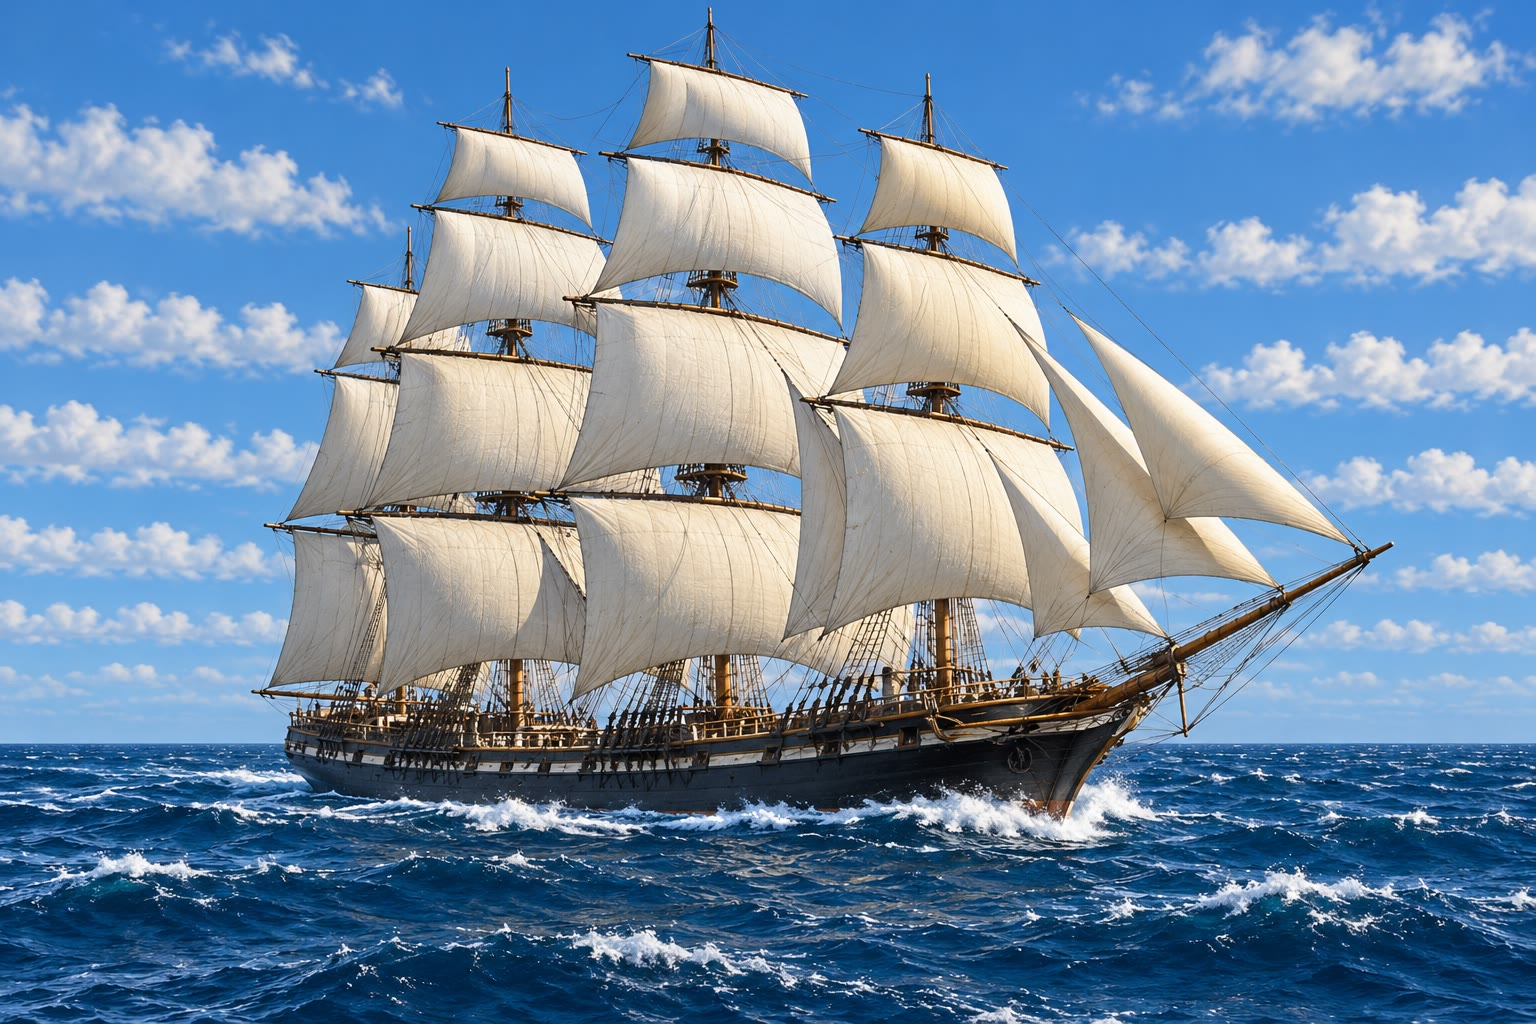
\includegraphics[width=0.62\linewidth]{images/book1/ai/g8-sailing-ship.jpg}

{\small Un voilier qui file vent arrière, poussé par un vent régulier, en
plein \omterm{def:g2:water-on-earth:ocean}{océan} (illustration générée par IA d'une scène générique).}
\label{fig:g8:winds-global-circulation:ship}
\end{omfigure}

Pourquoi l'alizé souffle-t-il de l'est, et toujours aux mêmes endroits~?
Pourquoi y a-t-il des \omterm{def:g5:weather-and-climate:desert}{déserts} près des \omterm{def:g5:weather-and-climate:tropics}{tropiques} et des \omterm{def:g5:weather-and-climate:rainforest}{forêts tropicales
humides} près de l'\omterm{def:g3:continents-and-oceans:equator}{équateur}~? La réponse commence avec le Soleil.

\begin{recall}
Le vent est de l'air en mouvement (les livres de physique). L'air appuie
sur tout ce qu'il touche, et la pression baisse avec l'\omterm{def:g4:world-physical-map:altitude}{altitude}
(\cref{ch:g8:the-atmosphere}). La \omterm{def:g1:watching-the-weather:weather}{météo} se produit dans la \omterm{def:g8:the-atmosphere:layers}{troposphère}, la
couche la plus basse de l'atmosphère. La Terre a des \omterm{def:g5:weather-and-climate:climate-zone}{zones climatiques}~:
chaudes et humides près de l'\omterm{def:g3:continents-and-oceans:equator}{équateur}, avec des \omterm{def:g5:weather-and-climate:rainforest}{forêts tropicales
humides}~; des \omterm{def:g5:weather-and-climate:desert}{déserts} chauds et secs près des \omterm{def:g5:weather-and-climate:tropics}{tropiques}~; des zones
tempérées, puis froides, vers les \omterm{def:g3:continents-and-oceans:poles}{pôles} (\cref{ch:g5:weather-and-climate}).
\end{recall}

\section{Le Soleil chauffe la Terre de façon inégale}

À midi, le jour d'un équinoxe, le Soleil est juste au-dessus de nos têtes
à l'\omterm{def:g3:continents-and-oceans:equator}{équateur}. Ses rayons y arrivent à la verticale et tombent sur une
petite surface de sol. Plus au nord ou plus au sud, les mêmes rayons
arrivent en biais et s'étalent sur une surface plus grande~: chaque mètre
carré reçoit moins de leur énergie. À la \omterm{def:g6:latitude-longitude:latitude}{latitude} \ang{60}, le même
faisceau couvre deux fois plus de sol qu'à l'\omterm{def:g3:continents-and-oceans:equator}{équateur}~: chaque mètre carré
en reçoit donc deux fois moins.
% ledger: (geometry: figdata/grade-8/sunlight_spread.py, spread = 1/cos(latitude))

\begin{omfigure}
\begin{tikzpicture}[font=\footnotesize]
  \def\R{2.6}\def\w{0.2}
  \fill[blue!10] (0,0) circle (\R);
  \draw (0,0) circle (\R);
  \draw[black!50] (-\R,0) -- (\R,0);
  \draw[black!40, dashed] (0,0) -- (60:\R);
  \draw[black!40] (0,0) ++(0:0.7) arc (0:60:0.7);
  \node at (25:0.95) {\ang{60}};
  \node[anchor=east, black!60] at (-\R-0.05,0) {équateur};
  % beam at the equator: rays between y = -w and y = w
  \foreach \y in {-0.2,-0.1,0,0.1,0.2} {
    \pgfmathsetmacro{\x}{sqrt(\R*\R-\y*\y)}
    \draw[orange!80!black, -{Stealth[length=1.6mm]}] (6.2,\y) -- (\x+0.03,\y);}
  \draw[omThm, line width=2.2pt] ({sqrt(\R*\R-0.35*0.35)},-0.35) arc ({asin(-\w/\R)}:{asin(\w/\R)}:\R);
  % beam near 60 degrees: rays between y = R sin 60 - w and + w
  \pgfmathsetmacro{\yc}{\R*sin(60)}
  \foreach \d in {-0.2,-0.1,0,0.1,0.2} {
    \pgfmathsetmacro{\y}{\yc+\d}
    \pgfmathsetmacro{\x}{sqrt(\R*\R-\y*\y)}
    \draw[orange!80!black, -{Stealth[length=1.6mm]}] (6.2,\y) -- (\x+0.03,\y);}
  \draw[omThm, line width=2.2pt] ({sqrt(\R*\R-(\yc-\w)^2)},\yc-\w) arc ({asin((\yc-\w)/\R)}:{asin((\yc+\w)/\R)}:\R);
  \node[anchor=west, align=left] at (6.3,0) {le même faisceau\\sur une petite surface};
  \node[anchor=west, align=left] at (6.3,\yc) {le même faisceau étalé\\sur deux fois plus de sol};
\end{tikzpicture}

{\small Deux faisceaux identiques de lumière du Soleil, à midi un jour
d'équinoxe. À l'\omterm{def:g3:continents-and-oceans:equator}{équateur}, ils tombent à la verticale sur une petite surface
(trait épais)~; à \ang{60} de \omterm{def:g6:latitude-longitude:latitude}{latitude}, ils arrivent en biais et couvrent
deux fois plus de sol.}
% ledger: (geometry: figdata/grade-8/sunlight_spread.py)
\label{fig:g8:winds-global-circulation:beams}
\end{omfigure}

\begin{center}\small
\begin{tabular}{|l|c|c|c|c|c|}
\hline
\omterm{def:g6:latitude-longitude:latitude}{latitude} & \ang{0} & \ang{30} & \ang{45} & \ang{60} & \ang{75} \\
\hline
sol couvert par le même faisceau & 1 & 1.15 & 1.41 & 2 & 3.86 \\
\hline
énergie par mètre carré (\% de celle de l'\omterm{def:g3:continents-and-oceans:equator}{équateur}) & 100 & 87 & 71 & 50 & 26 \\
\hline
\end{tabular}
\end{center}
% ledger: (figdata/grade-8/sunlight_spread.py main table)

Pendant que la Terre tourne autour du Soleil, son axe incliné fait passer
le Soleil de midi au zénith entre les deux \omterm{def:g5:weather-and-climate:tropics}{tropiques}, ce qui donne les
saisons (les livres de physique)~; mais toute l'année, les régions proches
de l'\omterm{def:g3:continents-and-oceans:equator}{équateur} reçoivent beaucoup plus d'énergie que celles qui sont
proches des \omterm{def:g3:continents-and-oceans:poles}{pôles}. Ce chauffage inégal est le principal moteur des
vents~: l'atmosphère transporte de l'air chaud vers les \omterm{def:g3:continents-and-oceans:poles}{pôles} et de l'air
froid vers l'\omterm{def:g3:continents-and-oceans:equator}{équateur}.
% ledger: mo:global-circ

\section{L'air qui monte et l'air qui descend}

L'air chaud est plus léger que l'air froid~: il monte, et l'air plus frais
qui l'entoure afflue pour prendre sa place. Là où l'air monte, il appuie
moins sur le sol~: la pression y est basse. Là où l'air descend, il
appuie davantage~: la pression est haute. Au sol, le vent souffle des
hautes pressions vers les basses pressions. En montant, en se refroidissant,
en descendant et en revenant, l'air tourne en boucle.
% ledger: jetstream:sea-breeze, mo:three-cells

\begin{definition}[Cellule de convection]\label{def:g8:winds-global-circulation:convection-cell}
Une \emph{cellule de convection}\index{cellule de convection} dans
l'atmosphère est une boucle d'air en mouvement~: l'air chauffé par le bas
monte, s'étale en \omterm{def:g4:world-physical-map:altitude}{altitude}, se refroidit et redescend ailleurs, puis
revient le long du sol jusqu'à l'endroit d'où il est monté. Sous l'air qui
monte, la pression est basse~; sous l'air qui descend, elle est haute.
\end{definition}
% ledger: jetstream:sea-breeze, mo:three-cells

\begin{inthelab}[L'air chaud monte]
À l'intérieur, découpe une spirale dans une feuille de papier fin, comme
l'épluchure d'une pomme, et suspends-la par son centre à un fil. Tiens-la
bien au-dessus d'un radiateur chaud, en hiver (jamais au-dessus d'une
flamme ou d'une bougie)~: elle se met lentement à tourner. L'air chauffé
par le radiateur monte et pousse sur la spirale. Tiens-la près d'une
fenêtre froide~: tourne-t-elle dans l'autre sens, ou plus du tout~?
\end{inthelab}

Les plus petites \omterm{def:g8:winds-global-circulation:convection-cell}{cellules de convection} se sentent un jour de soleil au
bord de la \omterm{def:g2:water-on-earth:ocean}{mer}. La terre et la \omterm{def:g2:water-on-earth:ocean}{mer} reçoivent le même soleil, mais les
rayons du Soleil ne pénètrent pas profondément dans le sol, tandis que la
\omterm{def:g2:water-on-earth:ocean}{mer} répartit sa chaleur dans une épaisse couche d'eau. La terre se
réchauffe donc beaucoup plus le jour, et se refroidit beaucoup plus la
nuit.
% ledger: jetstream:sea-breeze

\begin{omfigure}
\begin{tikzpicture}[font=\footnotesize, >={Stealth[length=2mm]}]
  \foreach \px/\title/\dir in {0/{Le jour~: la brise de mer}/1, 8.3/{La nuit~: la brise de terre}/-1} {
    \begin{scope}[xshift=\px cm]
      \fill[omSea] (0,0) rectangle (3.5,0.45);
      \fill[omLithAlluv] (3.5,0) -- (3.5,0.45) -- (7,0.75) -- (7,0) -- cycle;
      \draw (0,0.45) -- (3.5,0.45) -- (7,0.75);
      \node[anchor=south] at (3.5,3.25) {\textbf{\title}};
      \node at (1.75,0.22) {mer};
      \node at (5.6,0.3) {terre};
    \end{scope}}
  % day loop: surface sea -> land, rise over land, return aloft, sink over sea
  \draw[->, omDef, line width=1.1pt] (1.2,0.8) -- (5.2,0.95);
  \draw[->, omThm, line width=1.1pt] (5.8,1.1) -- (5.8,2.4);
  \draw[->, black!60, line width=1.1pt] (5.2,2.75) -- (1.2,2.75);
  \draw[->, omDef, line width=1.1pt] (0.6,2.4) -- (0.6,1.1);
  \node[omDef] at (3.2,1.25) {brise de mer};
  \node at (0.6,0.75) {\textbf{A}};
  \node at (5.8,0.95) {\textbf{D}};
  \fill[yellow!80!orange] (6.6,2.7) circle (0.25);
  \node[anchor=north, align=center] at (1.75,-0.1) {mer plus fraîche};
  \node[anchor=north, align=center] at (5.3,-0.1) {terre plus chaude};
  % night loop: surface land -> sea, rise over sea, return aloft, sink over land
  \begin{scope}[xshift=8.3cm]
    \draw[->, omDef, line width=1.1pt] (5.2,1.0) -- (1.2,0.8);
    \draw[->, omThm, line width=1.1pt] (0.6,1.1) -- (0.6,2.4);
    \draw[->, black!60, line width=1.1pt] (1.2,2.75) -- (5.2,2.75);
    \draw[->, omDef, line width=1.1pt] (5.8,2.4) -- (5.8,1.15);
    \node[omDef] at (3.2,1.3) {brise de terre};
    \node at (0.6,0.75) {\textbf{D}};
    \node at (5.8,1.0) {\textbf{A}};
    \fill[black!25] (6.6,2.7) circle (0.25); \fill[white] (6.72,2.78) circle (0.21);
    \node[anchor=north, align=center] at (1.75,-0.1) {mer plus chaude};
    \node[anchor=north, align=center] at (5.3,-0.1) {terre plus froide};
  \end{scope}
\end{tikzpicture}

{\small La \omterm{def:g8:winds-global-circulation:breezes}{brise de mer} et la \omterm{def:g8:winds-global-circulation:breezes}{brise de terre}~: deux petites \omterm{def:g8:winds-global-circulation:convection-cell}{cellules de
convection} qui tournent en sens contraires. Flèches rouges~: l'air chaud
qui monte~; A et D~: les hautes et les basses pressions au sol (A comme
anticyclone, D comme dépression). Le jour, la boucle monte jusqu'à 1000 à
\qty{1500}{m}.}
% ledger: jetstream:sea-breeze
\label{fig:g8:winds-global-circulation:breezes}
\end{omfigure}

\begin{definition}[Brise de mer et brise de terre]\label{def:g8:winds-global-circulation:breezes}
Une \emph{brise de mer}\index{brise de mer} est un vent qui souffle de la
\omterm{def:g2:water-on-earth:ocean}{mer} vers la terre le jour, quand la terre est plus chaude que la \omterm{def:g2:water-on-earth:ocean}{mer}. Une
\emph{brise de terre}\index{brise de terre} souffle de la terre vers la
\omterm{def:g2:water-on-earth:ocean}{mer} la nuit, quand la terre est devenue plus froide que la \omterm{def:g2:water-on-earth:ocean}{mer}.
\end{definition}
% ledger: jetstream:sea-breeze

\begin{omfigure}
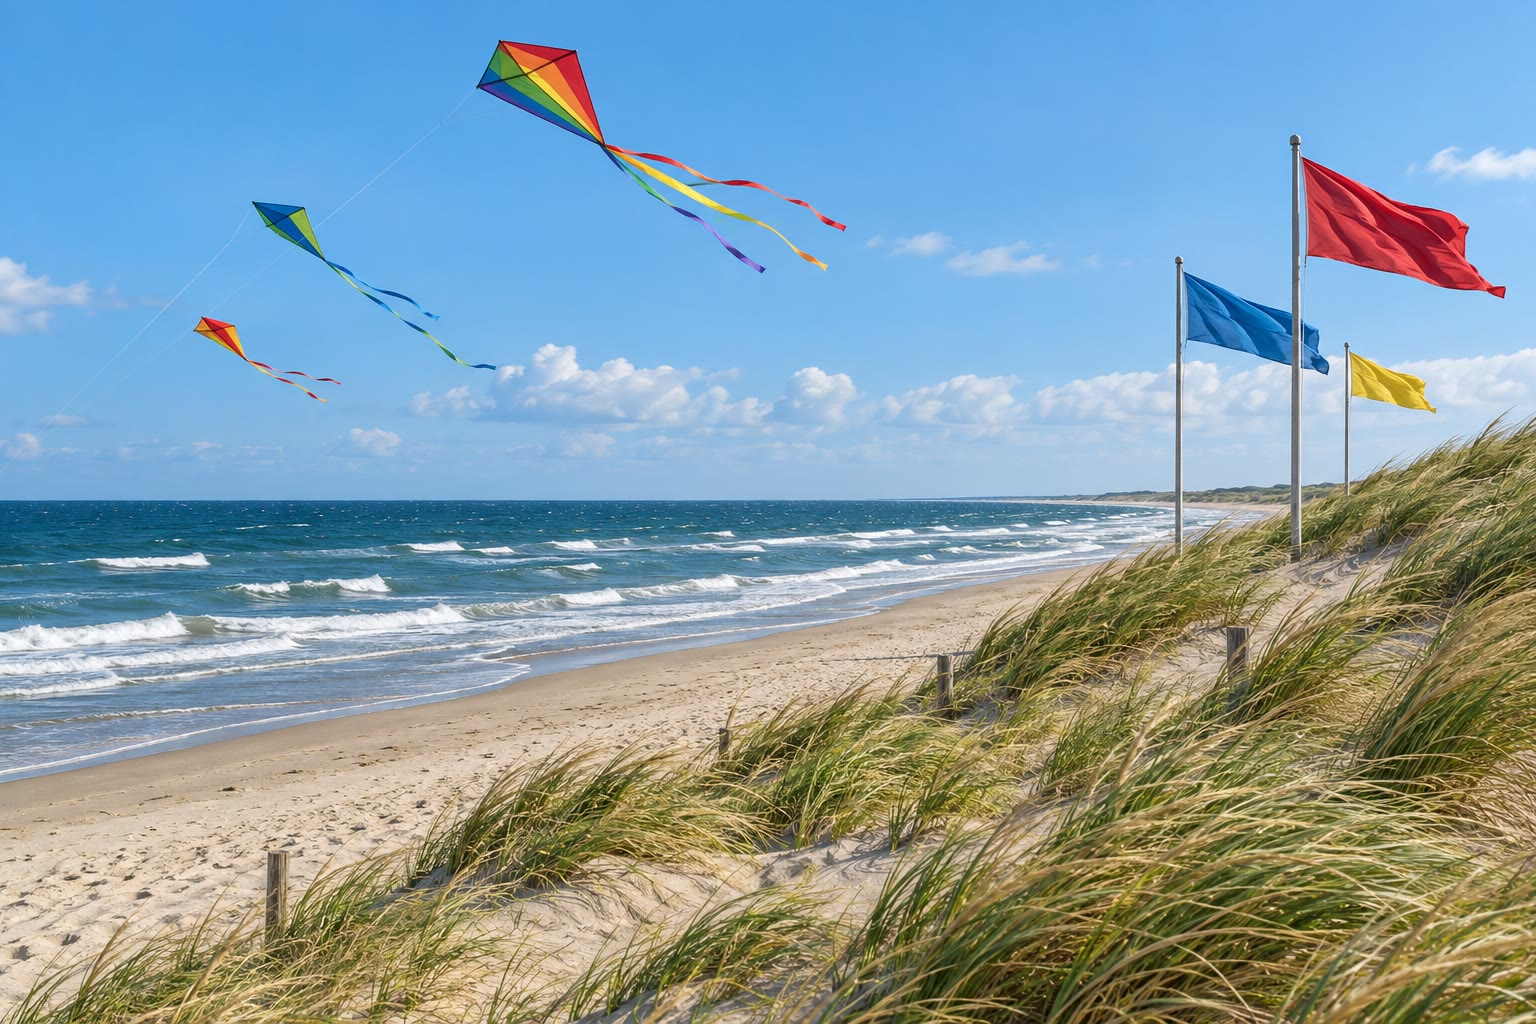
\includegraphics[width=0.55\linewidth]{images/book1/ai/g8-beach-kites.jpg}

{\small Des cerfs-volants dans le vent de l'après-midi, sur une plage
(illustration générée par IA d'une scène générique).}
\label{fig:g8:winds-global-circulation:kites}
\end{omfigure}

\section{Les vents de la planète}

La même chose se produit à l'échelle de la Terre entière. Près de
l'\omterm{def:g3:continents-and-oceans:equator}{équateur}, l'air fortement chauffé monte~; il s'étale vers les \omterm{def:g3:continents-and-oceans:poles}{pôles} en
\omterm{def:g4:world-physical-map:altitude}{altitude} et redescend vers \ang{30} de \omterm{def:g6:latitude-longitude:latitude}{latitude}. En moyenne sur de
nombreuses années, la \omterm{def:g8:the-atmosphere:layers}{troposphère} de chaque \omterm{def:g3:continents-and-oceans:equator}{hémisphère} tourne en trois
grandes \omterm{def:g8:winds-global-circulation:convection-cell}{cellules de convection}~: une de l'\omterm{def:g3:continents-and-oceans:equator}{équateur} jusque vers \ang{30},
une d'environ \ang{30} à environ \ang{60}, et une d'environ \ang{60}
jusqu'au \omterm{def:g3:continents-and-oceans:poles}{pôle}. Les météorologues les appellent les cellules de Hadley, de
Ferrel et polaires. Leurs limites se déplacent avec les saisons, et la
cellule du milieu est une moyenne grossière de nombreuses \omterm{def:g5:natural-hazards:storm}{tempêtes} qui
passent.
% ledger: mo:three-cells, mo:global-circ, nos:doldrums

Les vents qui soufflent au sol iraient tout droit des hautes vers les
basses pressions si la Terre ne tournait pas. Comme la Terre tourne, l'air
en mouvement est dévié~: vers la droite dans l'\omterm{def:g3:continents-and-oceans:equator}{hémisphère} Nord, vers la
gauche dans l'\omterm{def:g3:continents-and-oceans:equator}{hémisphère} Sud. L'air qui revient vers l'\omterm{def:g3:continents-and-oceans:equator}{équateur} ne vient
donc pas du nord, mais du nord-est dans l'\omterm{def:g3:continents-and-oceans:equator}{hémisphère} Nord, et du sud-est
dans l'\omterm{def:g3:continents-and-oceans:equator}{hémisphère} Sud.
% ledger: mo:global-circ, nos:trade-winds

\begin{definition}[Les vents de la planète]\label{def:g8:winds-global-circulation:global-winds}
Les vents de surface qui soufflent le plus souvent dans chaque bande de
\omterm{def:g6:latitude-longitude:latitude}{latitude} sont~:
\begin{itemize}
  \item les \emph{alizés}\index{alizes@alizés}, entre l'\omterm{def:g3:continents-and-oceans:equator}{équateur} et
        environ \ang{30}, qui soufflent du nord-est dans l'\omterm{def:g3:continents-and-oceans:equator}{hémisphère} Nord
        et du sud-est dans l'\omterm{def:g3:continents-and-oceans:equator}{hémisphère} Sud~;
  \item les \emph{vents d'ouest}\index{vents d'ouest}, entre environ
        \ang{30} et \ang{60}, qui soufflent de l'ouest (du sud-ouest dans
        l'\omterm{def:g3:continents-and-oceans:equator}{hémisphère} Nord, du nord-ouest dans l'\omterm{def:g3:continents-and-oceans:equator}{hémisphère} Sud)~;
  \item les \emph{vents d'est polaires}\index{vents d'est polaires}, entre
        environ \ang{60} et les \omterm{def:g3:continents-and-oceans:poles}{pôles}, qui soufflent de l'est.
\end{itemize}
\end{definition}
% ledger: nos:trade-winds, mo:three-cells, mo:global-circ

\begin{omfigure}
\begin{tikzpicture}[font=\scriptsize, >={Stealth[length=1.8mm]}]
  \def\R{3}
  \fill[blue!8] (0,0) circle (\R);
  \draw (0,0) circle (\R);
  \draw[black!45] (-\R,0) -- (\R,0);
  \foreach \l in {-60,-30,30,60} {
    \pgfmathsetmacro{\y}{\R*sin(\l)}
    \pgfmathsetmacro{\x}{\R*cos(\l)}
    \draw[black!45, dashed] (-\x,\y) -- (\x,\y);}
  % surface winds: NE trades, SW westerlies, NE polar easterlies (north); mirrored south
  \foreach \x in {-1.8,-0.6,0.6,1.8} {
    \draw[->, omThm, line width=0.9pt] (\x+0.35,0.95) -- (\x-0.35,0.55);
    \draw[->, omThm, line width=0.9pt] (\x+0.35,-0.95) -- (\x-0.35,-0.55);}
  \foreach \x in {-1.2,0,1.2} {
    \draw[->, omDef, line width=0.9pt] (\x-0.35,1.7) -- (\x+0.35,2.02);
    \draw[->, omDef, line width=0.9pt] (\x-0.35,-1.7) -- (\x+0.35,-2.02);}
  \foreach \x in {-0.4,0.4} {
    \draw[->, omMeth, line width=0.9pt] (\x+0.25,2.85) -- (\x-0.25,2.65);
    \draw[->, omMeth, line width=0.9pt] (\x+0.25,-2.85) -- (\x-0.25,-2.65);}
  \node[fill=blue!8, inner sep=1pt] at (0,1.2) {alizés du nord-est};
  \node[fill=blue!8, inner sep=1pt] at (0,-1.2) {alizés du sud-est};
  \node[fill=blue!8, inner sep=1pt] at (0,2.3) {vents d'ouest};
  \node[fill=blue!8, inner sep=1pt] at (0,-2.3) {vents d'ouest};
  \node[anchor=south] at (0,\R+0.05) {vents d'est polaires};
  \node[anchor=north] at (0,-\R-0.05) {vents d'est polaires};
  % pressure belts on the left
  \foreach \l/\t in {90/{A~: air qui descend}, 60/{D~: air qui monte}, 30/{A~: air qui descend, sec, déserts}, 0/{D~: air qui monte, nuages, pluie}, -30/{A~: air qui descend, sec, déserts}, -60/{D~: air qui monte}, -90/{A~: air qui descend}} {
    \pgfmathsetmacro{\y}{\R*sin(\l)}
    \pgfmathsetmacro{\x}{\R*cos(\l)}
    \draw[black!40] (-\x-0.05,\y) -- (-3.35,\y);
    \node[anchor=east] at (-3.4,\y) {\t};}
  \foreach \l/\t in {60/{\ang{60} N}, 30/{\ang{30} N}, 0/{équateur}, -30/{\ang{30} S}, -60/{\ang{60} S}} {
    \pgfmathsetmacro{\y}{\R*sin(\l)}
    \pgfmathsetmacro{\x}{\R*cos(\l)}
    \node[anchor=west, black!60] at (\x+0.05,\y) {\t};}
  % side view of the cells (height to the right), same latitude scale
  \begin{scope}[xshift=5.2cm]
    \draw[->] (0,-\R) -- (0,\R+0.3);
    \draw (0,-\R) -- (1.8,-\R);
    \node[anchor=north, align=center] at (0.9,-\R-0.05) {altitude dans la\\troposphère $\rightarrow$};
    \foreach \lo/\hi/\cw in {0/30/0, 30/60/1, 60/90/0, -30/0/1, -60/-30/0, -90/-60/1} {
      \pgfmathsetmacro{\ya}{\R*sin(\lo)}
      \pgfmathsetmacro{\yb}{\R*sin(\hi)}
      \pgfmathsetmacro{\yc}{(\ya+\yb)/2}
      \pgfmathsetmacro{\bb}{max(0.09,(\yb-\ya)/2-0.06)}
      \ifnum\cw=0
        \draw[black!70, line width=0.7pt, postaction={decorate}, decoration={markings,
          mark=at position 0.125 with {\arrow{Stealth[length=1.6mm]}}, mark=at position 0.375 with {\arrow{Stealth[length=1.6mm]}},
          mark=at position 0.625 with {\arrow{Stealth[length=1.6mm]}}, mark=at position 0.875 with {\arrow{Stealth[length=1.6mm]}}}]
          (0.9,\yc) ++(0.75,0) arc (0:360:0.75 and \bb);
      \else
        \draw[black!70, line width=0.7pt, postaction={decorate}, decoration={markings,
          mark=at position 0.125 with {\arrow{Stealth[length=1.6mm]}}, mark=at position 0.375 with {\arrow{Stealth[length=1.6mm]}},
          mark=at position 0.625 with {\arrow{Stealth[length=1.6mm]}}, mark=at position 0.875 with {\arrow{Stealth[length=1.6mm]}}}]
          (0.9,\yc) ++(0.75,0) arc (360:0:0.75 and \bb);
      \fi}
  \end{scope}
\end{tikzpicture}

{\small La \omterm{def:g8:winds-global-circulation:circulation}{circulation générale}, simplifiée. À gauche~: les bandes de
hautes (A) et de basses (D) pressions au sol. Sur le \omterm{def:g3:continents-and-oceans:globe}{globe}~: les vents de
surface, déviés par la rotation de la Terre. À droite~: les trois \omterm{def:g8:winds-global-circulation:convection-cell}{cellules
de convection} de chaque \omterm{def:g3:continents-and-oceans:equator}{hémisphère} vues de côté, aux mêmes \omterm{def:g6:latitude-longitude:latitude}{latitudes} (les
cellules polaires sont dessinées très minces parce que la bande polaire
est étroite sur le \omterm{def:g3:continents-and-oceans:globe}{globe}).}
% ledger: mo:three-cells, mo:global-circ, nos:trade-winds, nos:doldrums
\label{fig:g8:winds-global-circulation:cells}
\end{omfigure}

\begin{method}[Trouver le vent de la planète à une latitude]\label{met:g8:winds-global-circulation:wind}
\begin{enumerate}
  \item Trouve la bande~: de l'\omterm{def:g3:continents-and-oceans:equator}{équateur} jusque vers \ang{30}, de \ang{30}
        à \ang{60}, ou de \ang{60} jusqu'au \omterm{def:g3:continents-and-oceans:poles}{pôle}.
  \item Trouve dans quel sens l'air se déplace au sol dans cette bande~:
        vers l'\omterm{def:g3:continents-and-oceans:equator}{équateur} dans la première et la dernière bande, vers le \omterm{def:g3:continents-and-oceans:poles}{pôle}
        dans celle du milieu.
  \item Dévie ce mouvement~: vers la droite dans l'\omterm{def:g3:continents-and-oceans:equator}{hémisphère} Nord, vers
        la gauche dans l'\omterm{def:g3:continents-and-oceans:equator}{hémisphère} Sud.
  \item Dis d'où vient le vent~: les vents portent le nom de la direction
        \emph{d'où} ils soufflent.
\end{enumerate}
\end{method}

\begin{example}[Le vent à \ang{40} sud]\label{ex:g8:winds-global-circulation:40s}
À \ang{40} S, nous sommes dans la bande du milieu, entre \ang{30} et
\ang{60}. L'air y va, au sol, vers le \omterm{def:g3:continents-and-oceans:poles}{pôle}, c'est-à-dire vers le sud. Dans
l'\omterm{def:g3:continents-and-oceans:equator}{hémisphère} Sud, il est dévié vers la gauche~: pour de l'air qui va vers
le sud, la gauche est l'est~; l'air finit donc par se déplacer vers le
sud-est. Il vient donc du nord-ouest~: c'est l'un des \omterm{def:g8:winds-global-circulation:global-winds}{vents d'ouest}, qui
souffle du nord-ouest.
\end{example}
% ledger: mo:three-cells, mo:global-circ

Près de l'\omterm{def:g3:continents-and-oceans:equator}{équateur}, là où les \omterm{def:g8:winds-global-circulation:global-winds}{alizés} des deux \omterm{def:g3:continents-and-oceans:equator}{hémisphères} se rencontrent,
les vents faiblissent~: les marins appelaient cette bande de calme le
\emph{pot-au-noir}. L'air chaud et humide y monte, se refroidit et donne
des averses et des orages persistants. Vers \ang{30}, sous l'air qui
descend, les vents sont faibles et la \omterm{def:g4:clouds-rain-snow:precipitation}{pluie} est rare.
% ledger: nos:doldrums

\begin{definition}[Circulation générale de l'atmosphère]\label{def:g8:winds-global-circulation:circulation}
La \emph{circulation générale}\index{circulation generale@circulation générale} de
l'atmosphère est le mouvement de l'air à grande échelle autour de la
planète, tel qu'il apparaît quand on fait la moyenne des vents sur de
nombreuses années. Elle transporte de la chaleur de l'\omterm{def:g3:continents-and-oceans:equator}{équateur} vers les
\omterm{def:g3:continents-and-oceans:poles}{pôles}, et de la vapeur d'eau d'une bande de \omterm{def:g6:latitude-longitude:latitude}{latitude} à une autre.
\end{definition}
% ledger: mo:global-circ

\section{La circulation générale et les zones climatiques}

La \omterm{def:g8:winds-global-circulation:circulation}{circulation générale} explique une grande partie de la \omterm{def:g2:drawing-to-map:map}{carte} des
\omterm{def:g5:weather-and-climate:climate}{climats}. Là où l'air monte, près de l'\omterm{def:g3:continents-and-oceans:equator}{équateur}, il se refroidit et sa
vapeur d'eau se change en \omterm{def:g4:clouds-rain-snow:cloud}{nuages}~: la \omterm{def:g4:clouds-rain-snow:precipitation}{pluie} est fréquente, et des \omterm{def:g5:weather-and-climate:rainforest}{forêts
tropicales humides} poussent. Là où l'air descend, vers \ang{30} nord et
sud, il se réchauffe en descendant, ses \omterm{def:g4:clouds-rain-snow:cloud}{nuages} se dissipent, et la \omterm{def:g4:clouds-rain-snow:precipitation}{pluie}
est rare~: les grands \omterm{def:g5:weather-and-climate:desert}{déserts} chauds, comme le Sahara, se trouvent dans
ces bandes. Aux \omterm{def:g6:latitude-longitude:latitude}{latitudes} moyennes, les \omterm{def:g8:winds-global-circulation:global-winds}{vents d'ouest} amènent une \omterm{def:g5:natural-hazards:storm}{tempête}
après l'autre, avec de la \omterm{def:g4:clouds-rain-snow:precipitation}{pluie} en toute saison.
% ledger: nos:doldrums, mo:three-cells, mo:global-circ

\begin{omfigure}
\begin{minipage}[c]{0.42\linewidth}\centering
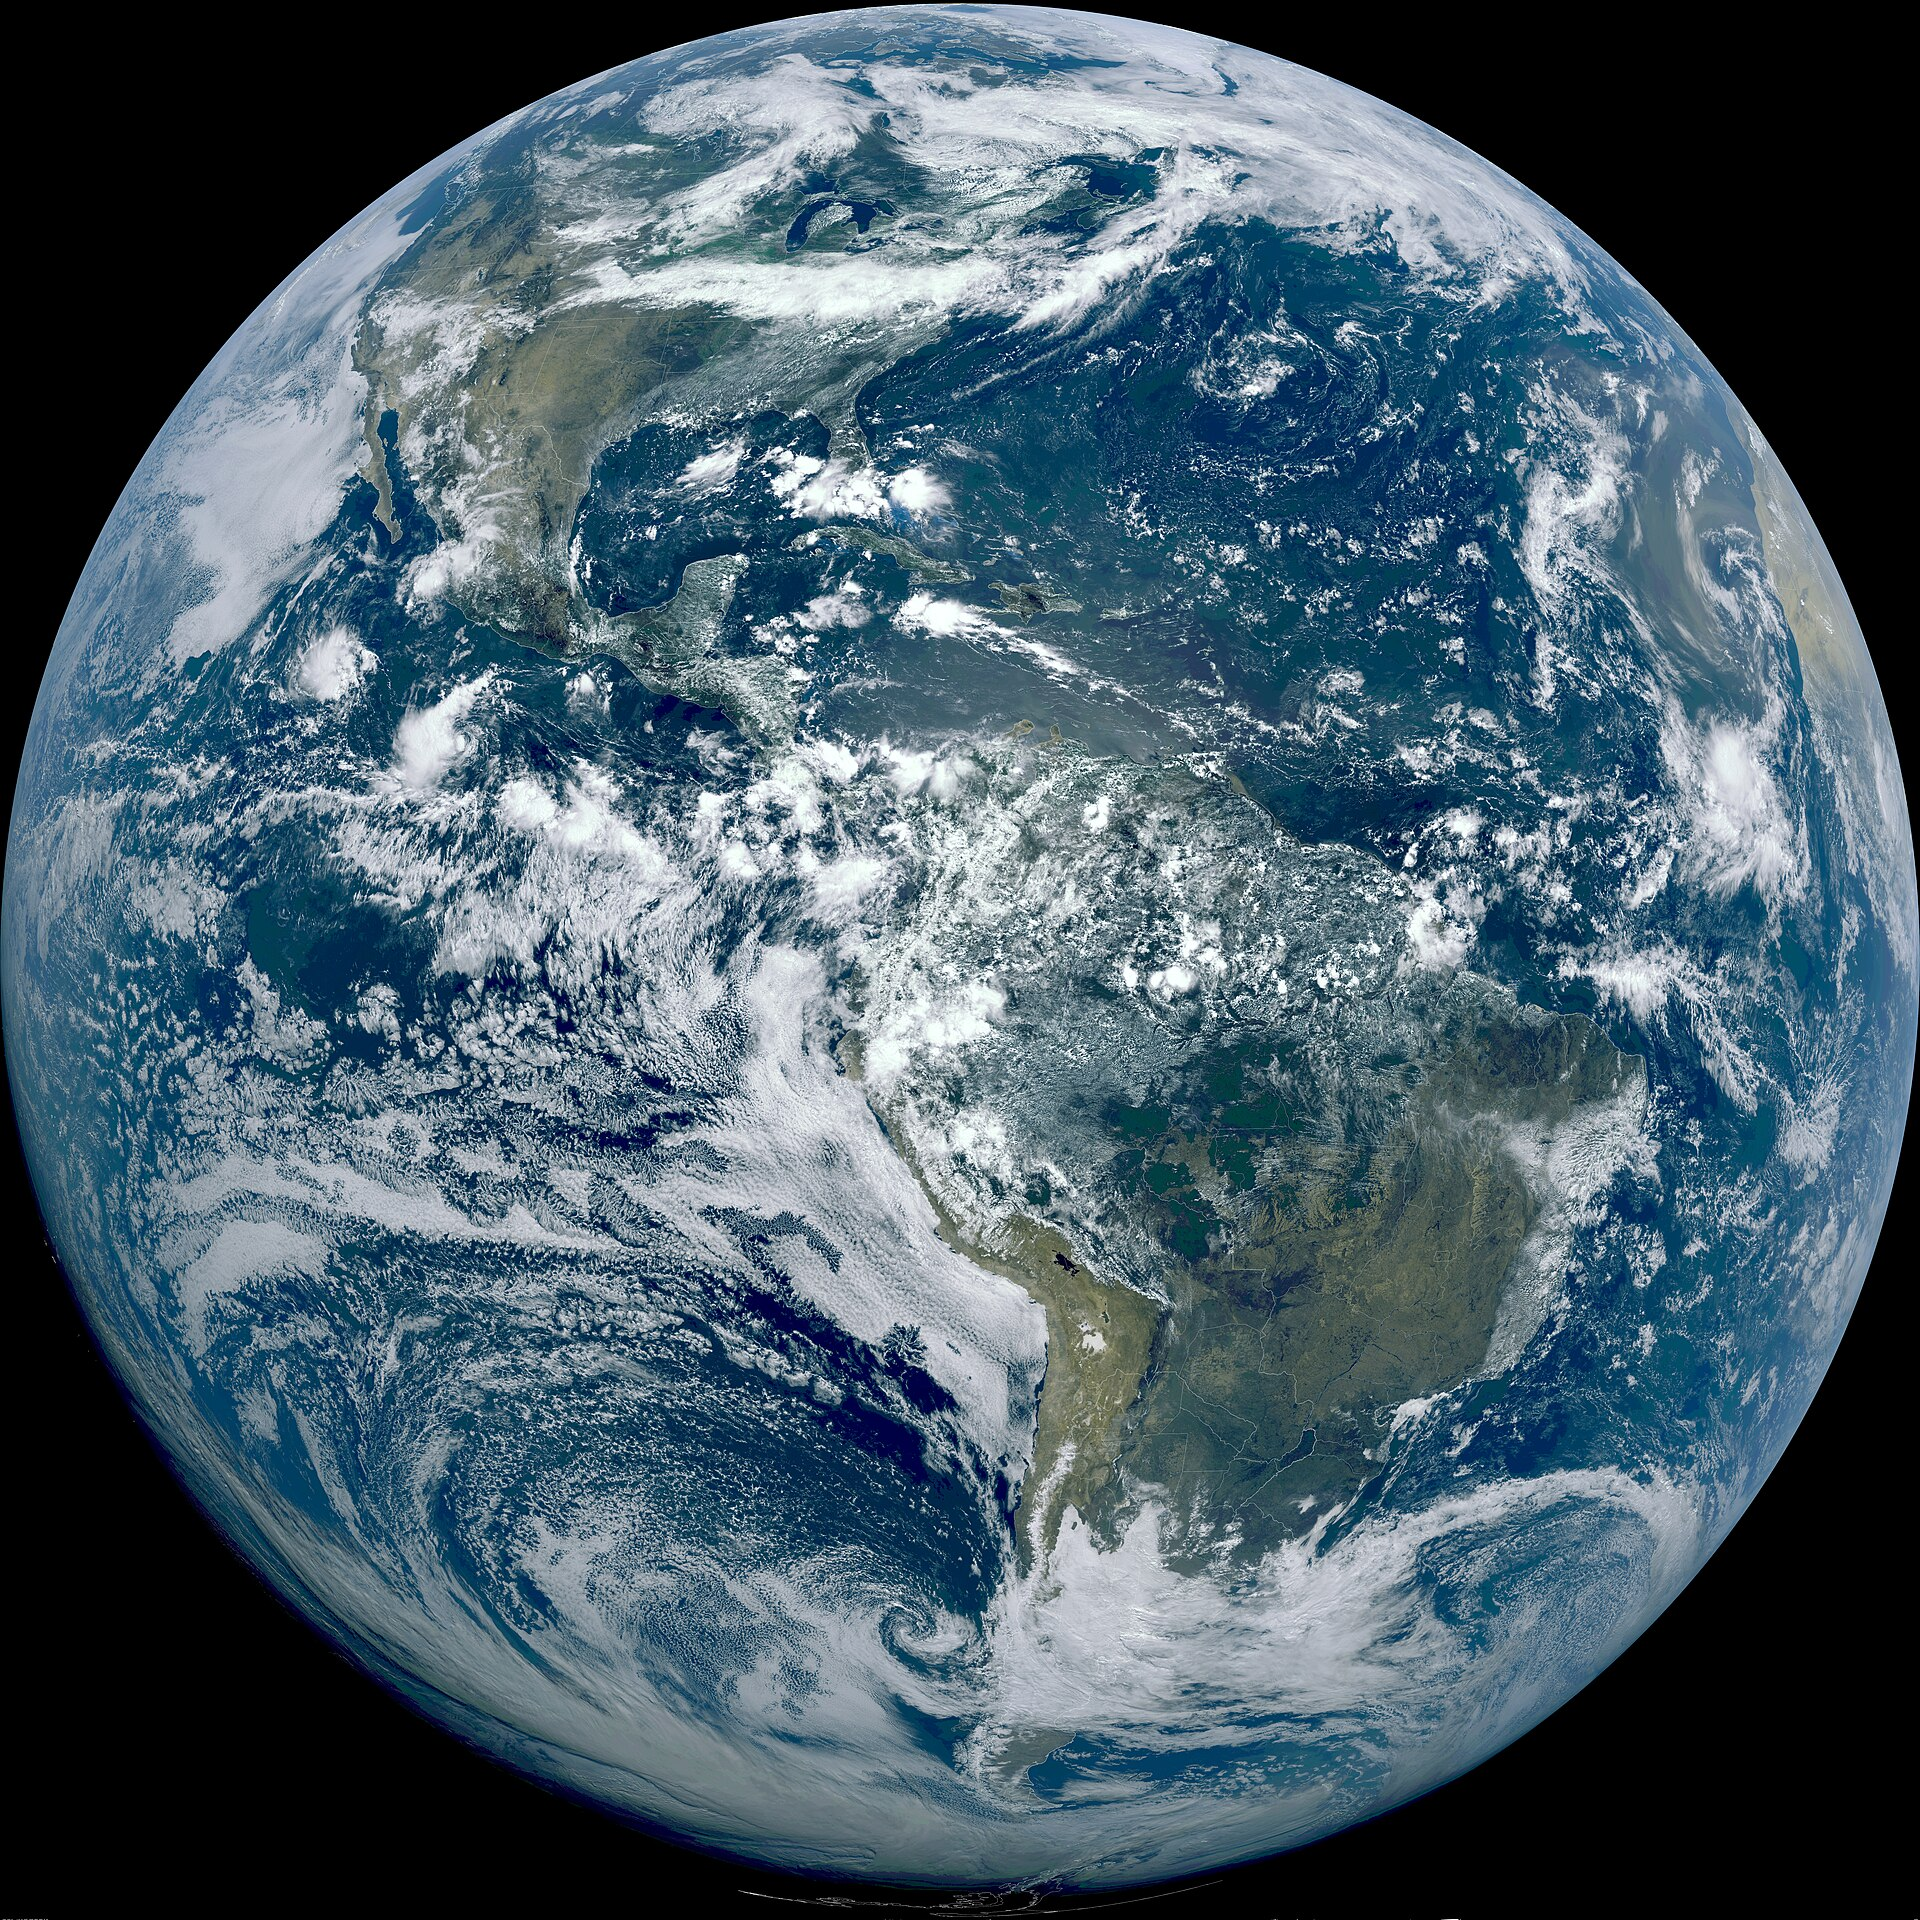
\includegraphics[width=\linewidth]{images/book1/g8-goes-full-disk.jpg}
\end{minipage}\hfill
\begin{minipage}[c]{0.54\linewidth}\raggedright
{\small Les Amériques vues par le satellite \omterm{def:g1:watching-the-weather:weather}{météorologique} GOES-16, très
haut au-dessus de l'\omterm{def:g3:continents-and-oceans:equator}{équateur}, le 26~juillet 2022. De nombreux \omterm{def:g4:clouds-rain-snow:cloud}{nuages} se
sont formés au-dessus des \omterm{def:g5:weather-and-climate:tropics}{tropiques} et de la forêt amazonienne, où l'air
chaud et humide monte~; loin vers le sud, pendant l'hiver austral, les
\omterm{def:g5:natural-hazards:storm}{tempêtes} des \omterm{def:g8:winds-global-circulation:global-winds}{vents d'ouest} tourbillonnent au-dessus de l'\omterm{def:g2:water-on-earth:ocean}{océan}. NOAA
(domaine public, via Wikimedia Commons).}
\end{minipage}
% ledger: commons:goes16, nos:doldrums
\label{fig:g8:winds-global-circulation:goes}
\end{omfigure}

\begin{example}[Quatre villes, quatre bandes]\label{ex:g8:winds-global-circulation:four-towns}
Les quatre villes des \omterm{def:g5:weather-and-climate:climate-chart}{diagrammes climatiques} du
\cref{ch:g5:weather-and-climate} se trouvent toutes dans l'\omterm{def:g3:continents-and-oceans:equator}{hémisphère} Nord,
à des \omterm{def:g6:latitude-longitude:latitude}{latitudes} très différentes. Leurs \omterm{def:g4:clouds-rain-snow:precipitation}{précipitations} annuelles suivent
les bandes de la \omterm{def:g8:winds-global-circulation:circulation}{circulation générale} (graphique ci-dessous). Hilo, à
\ang{20}\,N, est sur une île de la bande des \omterm{def:g8:winds-global-circulation:global-winds}{alizés}, au milieu de
l'\omterm{def:g2:water-on-earth:ocean}{océan}, où les \omterm{def:g8:winds-global-circulation:global-winds}{alizés} se chargent de vapeur d'eau~: il y tombe environ
\qty{3000}{mm} par an. Phoenix, à \ang{33}\,N, est proche de \ang{30},
sous l'air qui descend~: moins de \qty{200}{mm}. Seattle, à \ang{47}\,N,
est dans les \omterm{def:g8:winds-global-circulation:global-winds}{vents d'ouest}, dont les \omterm{def:g5:natural-hazards:storm}{tempêtes} apportent environ
\qty{1000}{mm} par an, surtout de l'automne au printemps. Utqiaġvik, à
\ang{71}\,N, se trouve sous l'air froid qui descend près du \omterm{def:g3:continents-and-oceans:poles}{pôle}~: moins
de \qty{150}{mm}, un \omterm{def:g5:weather-and-climate:desert}{désert} froid.
% ledger: data:b1-noaa-normals (totals from figdata/grade-5/climate_charts.py, re-read in figdata/grade-8/rain_by_belt.py), mo:three-cells, nos:doldrums
\end{example}

\begin{omfigure}
\begin{tikzpicture}
\begin{axis}[xbar, width=0.82\linewidth, height=6.4cm, bar width=9pt,
  xmin=0, xmax=3600, ymin=0, ymax=90, ytick={0,30,60,90},
  yticklabels={$0^\circ$, $30^\circ$\,N, $60^\circ$\,N, $90^\circ$\,N},
  xlabel={pluie et neige en un an (mm)}, ylabel={latitude},
  axis x line=bottom, axis y line=left, axis line style={-},
  tick label style={font=\scriptsize}, label style={font=\small},
  xtick={0,1000,2000,3000}, scaled x ticks=false, clip=false,
  point meta=explicit symbolic, nodes near coords,
  nodes near coords style={font=\scriptsize, anchor=west}]
  \draw[black!35, dashed] (axis cs:0,30) -- (axis cs:3600,30);
  \draw[black!35, dashed] (axis cs:0,60) -- (axis cs:3600,60);
  \node[font=\scriptsize, black!60, anchor=south east] at (axis cs:3600,1) {air qui monte~: pluie};
  \node[font=\scriptsize, black!60, anchor=south east] at (axis cs:3600,30) {air qui descend~: sec};
  \node[font=\scriptsize, black!60, anchor=south east] at (axis cs:3600,60) {air qui monte~: pluie};
  \node[font=\scriptsize, black!60, anchor=north east] at (axis cs:3600,90) {air qui descend~: sec};
  \addplot[fill=blue!35, draw=blue!60!black] table[x=total_mm, y=lat, meta=name] {figdata/out/grade-8-rain_by_belt-stations.dat};
\end{axis}
\end{tikzpicture}

{\small \omterm{def:g4:clouds-rain-snow:precipitation}{Précipitations} annuelles (moyennes 1991--2020) des quatre villes
des \omterm{def:g5:weather-and-climate:climate-chart}{diagrammes climatiques}, placées à leur \omterm{def:g6:latitude-longitude:latitude}{latitude}. Les villes humides se
trouvent là où l'air monte, près de l'\omterm{def:g3:continents-and-oceans:equator}{équateur} et vers \ang{60}~; les
villes sèches là où il descend, vers \ang{30} et près du \omterm{def:g3:continents-and-oceans:poles}{pôle}. Normales
climatiques de la NOAA.}
% ledger: data:b1-noaa-normals, mo:three-cells (figdata/grade-8/rain_by_belt.py)
\end{omfigure}

Quatre villes ne sont que quatre points~: les \omterm{def:g1:landscapes-around-us:landform}{montagnes}, les \omterm{def:g1:landscapes-around-us:water}{côtes} et les
\omterm{def:g2:water-on-earth:ocean}{mers} froides ou chaudes changent aussi la quantité de \omterm{def:g4:clouds-rain-snow:precipitation}{pluie} que reçoit un
lieu. Les bandes donnent le dessin d'ensemble de la \omterm{def:g2:drawing-to-map:map}{carte} des \omterm{def:g5:weather-and-climate:climate}{climats}, pas
la \omterm{def:g4:clouds-rain-snow:precipitation}{pluie} de chaque ville.

\section{Exercices}

\begin{exercise}[$\star$]\label{exo:g8:winds-global-circulation:1}
Nomme le vent de la planète qui souffle le plus souvent~: (a) à \ang{15}
nord~; (b) à \ang{45} sud~; (c) à \ang{75} nord~; (d) à \ang{20} sud.
Donne chaque fois sa direction.
\end{exercise}

\begin{exercise}[$\star$]\label{exo:g8:winds-global-circulation:2}
Complète chaque phrase. (a) L'air chaud \dots\ et l'air froid \dots. (b)
Sous l'air qui monte, la pression au sol est \dots. (c) Au sol, le vent
souffle des \dots\ pressions vers les \dots\ pressions. (d) Dans
l'\omterm{def:g3:continents-and-oceans:equator}{hémisphère} Nord, la rotation de la Terre dévie l'air en mouvement vers
la \dots.
\end{exercise}

\begin{exercise}[$\star$]\label{exo:g8:winds-global-circulation:3}
Vrai ou faux~? Corrige les phrases fausses. (a) Une \omterm{def:g8:winds-global-circulation:breezes}{brise de mer} souffle
de la terre vers la \omterm{def:g2:water-on-earth:ocean}{mer}. (b) Le jour, la terre se réchauffe plus vite que
la \omterm{def:g2:water-on-earth:ocean}{mer}. (c) Les \omterm{def:g8:winds-global-circulation:global-winds}{alizés} soufflent de l'ouest. (d) Beaucoup de grands
\omterm{def:g5:weather-and-climate:desert}{déserts} se trouvent vers \ang{30} de \omterm{def:g6:latitude-longitude:latitude}{latitude}.
\end{exercise}

\begin{exercise}[$\star$]\label{exo:g8:winds-global-circulation:4}
Dessine une \omterm{def:g1:landscapes-around-us:water}{côte} avec la \omterm{def:g2:water-on-earth:ocean}{mer} à gauche et la terre à droite. Ajoute le
Soleil, puis dessine avec des flèches la boucle d'air de la \omterm{def:g8:winds-global-circulation:breezes}{brise de mer}.
Marque A et D là où la pression au sol est haute et basse.
\end{exercise}

\begin{exercise}[$\star\star$]\label{exo:g8:winds-global-circulation:5}
Utilise le tableau des faisceaux de ce chapitre. (a) À \ang{45}, combien
de sol un faisceau couvre-t-il de plus qu'à l'\omterm{def:g3:continents-and-oceans:equator}{équateur}~? (b) Quel
pourcentage de l'énergie de l'\omterm{def:g3:continents-and-oceans:equator}{équateur} chaque mètre carré reçoit-il à
\ang{60}~? (c) À \ang{75}~? (d) Explique en une phrase pourquoi il fait
froid aux \omterm{def:g3:continents-and-oceans:poles}{pôles}.
\end{exercise}

\begin{exercise}[$\star\star$]\label{exo:g8:winds-global-circulation:6}
Un bateau navigue plein sud à travers l'\omterm{def:g3:continents-and-oceans:equator}{hémisphère} Nord, puis
l'\omterm{def:g3:continents-and-oceans:equator}{hémisphère} Sud. (a) Quels vents rencontre-t-il, dans l'ordre, de
\ang{70} N à \ang{70} S~? (b) Où risque-t-il de trouver un air calme et
des averses fréquentes~? (c) Où les vents sont-ils faibles et la \omterm{def:g4:clouds-rain-snow:precipitation}{pluie}
rare~?
\end{exercise}

\begin{exercise}[$\star\star$]\label{exo:g8:winds-global-circulation:7}
Sur une plage, il fait \qty{31}{\degreeCelsius} sur le \omterm{def:g3:stones-pebbles-sand:sand}{sable} à 15~h et
\qty{22}{\degreeCelsius} au-dessus de la \omterm{def:g2:water-on-earth:ocean}{mer}. À 3~h du matin, il fait
\qty{17}{\degreeCelsius} sur la terre et \qty{21}{\degreeCelsius}
au-dessus de la \omterm{def:g2:water-on-earth:ocean}{mer}. (a) Qu'est-ce qui est le plus chaud à 15~h~? Dans
quel sens souffle le vent~? (b) Et à 3~h du matin~? (c) De combien de
degrés la température de la terre change-t-elle entre ces deux moments~?
Et celle de la \omterm{def:g2:water-on-earth:ocean}{mer}~? (d) Explique la différence.
\end{exercise}

\begin{exercise}[$\star\star$]\label{exo:g8:winds-global-circulation:8}
L'air s'écoule de la bande de hautes pressions située vers \ang{30} N vers
l'\omterm{def:g3:continents-and-oceans:equator}{équateur}. (a) Sans la rotation de la Terre, de quelle direction
soufflerait-il~? (b) De quel côté la rotation le dévie-t-elle dans cet
\omterm{def:g3:continents-and-oceans:equator}{hémisphère}~? (c) De quelle direction souffle-t-il alors~? (d) Réponds aux
trois mêmes questions pour l'air qui s'écoule vers l'\omterm{def:g3:continents-and-oceans:equator}{équateur} depuis
\ang{30} S.
\end{exercise}

\begin{exercise}[$\star\star$]\label{exo:g8:winds-global-circulation:9}
Explique, étape par étape, pourquoi il pleut si souvent près de
l'\omterm{def:g3:continents-and-oceans:equator}{équateur}~: utilise les mots \emph{chauffé}, \emph{monte}, \emph{se refroidit}, \emph{\omterm{def:g4:clouds-rain-snow:cloud}{nuages}}.
Explique ensuite pourquoi il y a un \omterm{def:g5:weather-and-climate:desert}{désert} vers \ang{25} N en Afrique du
Nord~: utilise les mots \emph{descend}, \emph{hautes pressions}, \emph{sec}.
\end{exercise}

\begin{exercise}[$\star\star$]\label{exo:g8:winds-global-circulation:10}
Un voilier quitte un port situé à \ang{40} N, sur la \omterm{def:g1:landscapes-around-us:water}{côte} ouest de
l'Europe, pour les Caraïbes, à \ang{15} N. (a) Quel vent rencontrerait-il
à \ang{40} N~? L'aiderait-il à naviguer vers l'ouest~? (b) Pourquoi le
navire devrait-il d'abord descendre vers le sud~? (c) Quel vent le pousse
vers l'ouest, et entre quelles \omterm{def:g6:latitude-longitude:latitude}{latitudes}~? (d) Pour le voyage de retour
vers l'Europe, quel vent le navire devrait-il chercher, et à quelle
\omterm{def:g6:latitude-longitude:latitude}{latitude}~?
\end{exercise}

\begin{exercise}[$\star\star\star$]\label{exo:g8:winds-global-circulation:11}
À la \omterm{def:g6:latitude-longitude:latitude}{latitude} $L$, un faisceau de lumière du Soleil, à midi un jour
d'équinoxe, couvre $1 \div
\cos L$ fois le sol qu'il couvre à l'\omterm{def:g3:continents-and-oceans:equator}{équateur} (à la calculatrice,
$\cos 60^\circ = 0.5$). (a) Vérifie la valeur pour \ang{60}. (b) Avec
$\cos 30^\circ \approx 0.866$, vérifie la valeur pour \ang{30}, arrondie
au centième. (c) Suppose qu'un panneau solaire posé à plat reçoive
\qty{1000}{W} sur chaque mètre carré à midi, à l'\omterm{def:g3:continents-and-oceans:equator}{équateur}, ce jour-là.
Environ combien le même panneau recevrait-il à \ang{30}~? À \ang{60}~?
\end{exercise}

\begin{exercise}[$\star\star\star$]\label{exo:g8:winds-global-circulation:12}
Dans chaque \omterm{def:g3:continents-and-oceans:equator}{hémisphère}, la \omterm{def:g8:winds-global-circulation:circulation}{circulation générale} compte trois cellules.
(a) Dessine une vue de côté de l'\omterm{def:g3:continents-and-oceans:equator}{hémisphère} Nord, avec l'\omterm{def:g3:continents-and-oceans:equator}{équateur} en bas
et le \omterm{def:g3:continents-and-oceans:poles}{pôle} en haut, et les trois cellules sous forme de boucles~; montre
où l'air monte et où il descend. (b) Marque les bandes de hautes et de
basses pressions au sol. (c) Ajoute les vents de surface de chaque
cellule, déviés vers la droite. (d) Sers-toi de ton dessin pour expliquer
pourquoi les \omterm{def:g8:winds-global-circulation:global-winds}{vents d'ouest} soufflent vers le nord-est.
\end{exercise}

\section{Problème~: Naviguer avec les alizés}

\begin{problem}[{Problème du week-end --- un voilier traverse l'Atlantique
du Cap-Vert à la Barbade avec l'alizé du nord-est~; la route est mesurée
sur la carte, le vent est lu, et l'on calcule la durée de la
traversée}]
\label{pb:g8:winds-global-circulation:1}
% ledger: data:b1-ne-places, earth:Rmean, nos:trade-winds (figdata/grade-8/trade_route.py; the speed is exercise data)
Un voilier quitte Praia, dans les îles du Cap-Vert, pour Bridgetown, à la
Barbade. La \omterm{def:g2:drawing-to-map:map}{carte} montre la route et l'alizé.

\begin{center}
\begin{tikzpicture}
\begin{axis}[ommap, width=12cm, xmin=-75, xmax=-5, ymin=0, ymax=35, axis equal image,
  xtick={-70,-60,-50,-40,-30,-20,-10}, ytick={0,10,20,30},
  tick label style={font=\scriptsize},
  xlabel={longitude (négative = ouest)}, ylabel={latitude (nord)},
  label style={font=\small}, clip mode=individual]
  \addplot[fill=omLithAlluv, draw=black!60, line width=0.3pt] table {figdata/out/grade-8-trade_route-land.dat};
  \addplot[quiver={u=\thisrow{dlon}, v=\thisrow{dlat}}, -{Stealth[length=1.6mm]}, omThm!80, line width=0.7pt]
    table[x=lon, y=lat] {figdata/out/grade-8-trade_route-trades.dat};
  \addplot[omDef, line width=1.3pt, dashed] table {figdata/out/grade-8-trade_route-route.dat};
  \addplot[only marks, mark=*, mark size=2pt, black] table[x=lon, y=lat] {figdata/out/grade-8-trade_route-ports.dat};
  \node[anchor=north, font=\scriptsize\bfseries, fill=white, inner sep=1pt] at (axis cs:-59.6,12.2) {Bridgetown};
  \node[anchor=south, font=\scriptsize\bfseries, fill=white, inner sep=1pt] at (axis cs:-23.5,15.8) {Praia};
\end{axis}
\end{tikzpicture}
\end{center}

\noindent\textbf{Partie I --- La route.}\par\nopagebreak
\begin{enumerate}[beginpenalty=10000]
  \item Praia se trouve à \ang{14.9} N, \ang{23.5} O~; Bridgetown à
        \ang{13.1} N, \ang{59.6} O. Combien de degrés de \omterm{def:g6:latitude-longitude:longitude}{longitude} les
        séparent~?
  \item Les deux ports se trouvent près de \ang{14} N. Le long de ce
        \omterm{def:g6:latitude-longitude:latitude}{parallèle}, un degré de \omterm{def:g6:latitude-longitude:longitude}{longitude} mesure environ \qty{108}{km}.
        Environ combien de kilomètres mesure la traversée~? Arrondis à la
        centaine.
  \item Mesurée exactement sur la Terre ronde, la route la plus courte
        mesure \qty{3896}{km}. La réponse à la question 2 est-elle une
        bonne estimation~?
  \item Les ports se trouvent-ils dans la bande des \omterm{def:g8:winds-global-circulation:global-winds}{alizés}~? Explique.
\end{enumerate}

\noindent\textbf{Partie II --- Le vent.}\par\nopagebreak
\begin{enumerate}[resume, beginpenalty=10000]
  \item De quelle direction souffle l'alizé ici~?
  \item Le voilier navigue vers l'ouest. Le vent le pousse-t-il vers
        l'avant, vers l'arrière ou sur le côté~? Explique avec la \omterm{def:g2:drawing-to-map:map}{carte}.
  \item Pourquoi l'alizé souffle-t-il dans la même direction presque
        chaque jour de la traversée~?
  \item Pour le retour vers l'Europe, pourquoi le capitaine ne doit-il pas
        essayer de naviguer vers l'est le long de \ang{14} N~?
\end{enumerate}

\noindent\textbf{Partie III --- La traversée.}\par\nopagebreak
\begin{enumerate}[resume, beginpenalty=10000]
  \item Suppose que le voilier avance en moyenne à \qty{7}{km} par heure.
        Combien de kilomètres parcourt-il en une journée de 24~heures~?
  \item Si le vent tombait pendant 3~jours en route, combien de
        kilomètres de progression le voilier perdrait-il~?
  \item Avec un alizé régulier, combien de jours faut-il au voilier pour
        \qty{3896}{km}~? Arrondis au dixième.
  \item Au jour près, combien de temps dure la traversée~? Est-ce plus ou
        moins d'un mois~?
\end{enumerate}
\end{problem}
